\section{The \pate{} Binary Ninja Plugin}
\label{sec:binary-ninja-ui}

The \pate{} Binary Ninja plugin enables user to invoke and interact with \pate{} directly within the Binary Ninja reverse engineering platform.

The \pate{} plugin requires a commercially-licensed Binary Ninja installation.
We have tested \pate{} with Binary Ninja stable version 4.0.5336.

\subsection{Installation}

First, install the \pate{} Docker container as described in Section~\ref{sec:build-pate-verif}.

Second, copy (or create a symlink from) the \texttt{pate\_binja/} directory from the \pate{} source repo to your local Binary Ninja \texttt{plugins/} directory. Typically these are found in:
\begin{description}
\item[macOS] \texttt{\$HOME/Library/Application Support/Binary Ninja/plugins/}
\item[Linux] \texttt{\$HOME/.binaryninja/plugins/}
\end{description}

The Binary Ninja plugin requires a relatively recent version of Python (3.10 or newer) and requires the \texttt{grpcio} package.
If these are not present on the system, we recommend creating a Python \texttt{venv} or similar on your host, with something like:

\begin{verbatim}
  python -m venv /path/to/new/virtual/environment
  source /path/to/new/virtual/environment/bin/activate
  pip install grpcio
\end{verbatim}

and then modifying Binary Ninja Python settings appropriately in the Binary Ninja Preferences list to point to this new environment.
Specifically, check the settings for:

\begin{itemize}
    \item Python Path Override
    \item Python Interpreter
    \item Python Virtual Environment Site-Packages
\end{itemize}

Once these steps have been completed, restart Binary Ninja.
If the plugin is correctly installed and initialized, then the ``Plugins'' menu will now have a ``Pate...'' menu option.

\subsection{Usage}

In Section~\ref{sec:terminal-ui} we examined the \texttt{packet.exe} example using the \pate{} terminal UI.
In this section, we describe analyzing the same example using the \pate{} Binary Ninja plugin.

\begin{figure}[h]
  \centering
  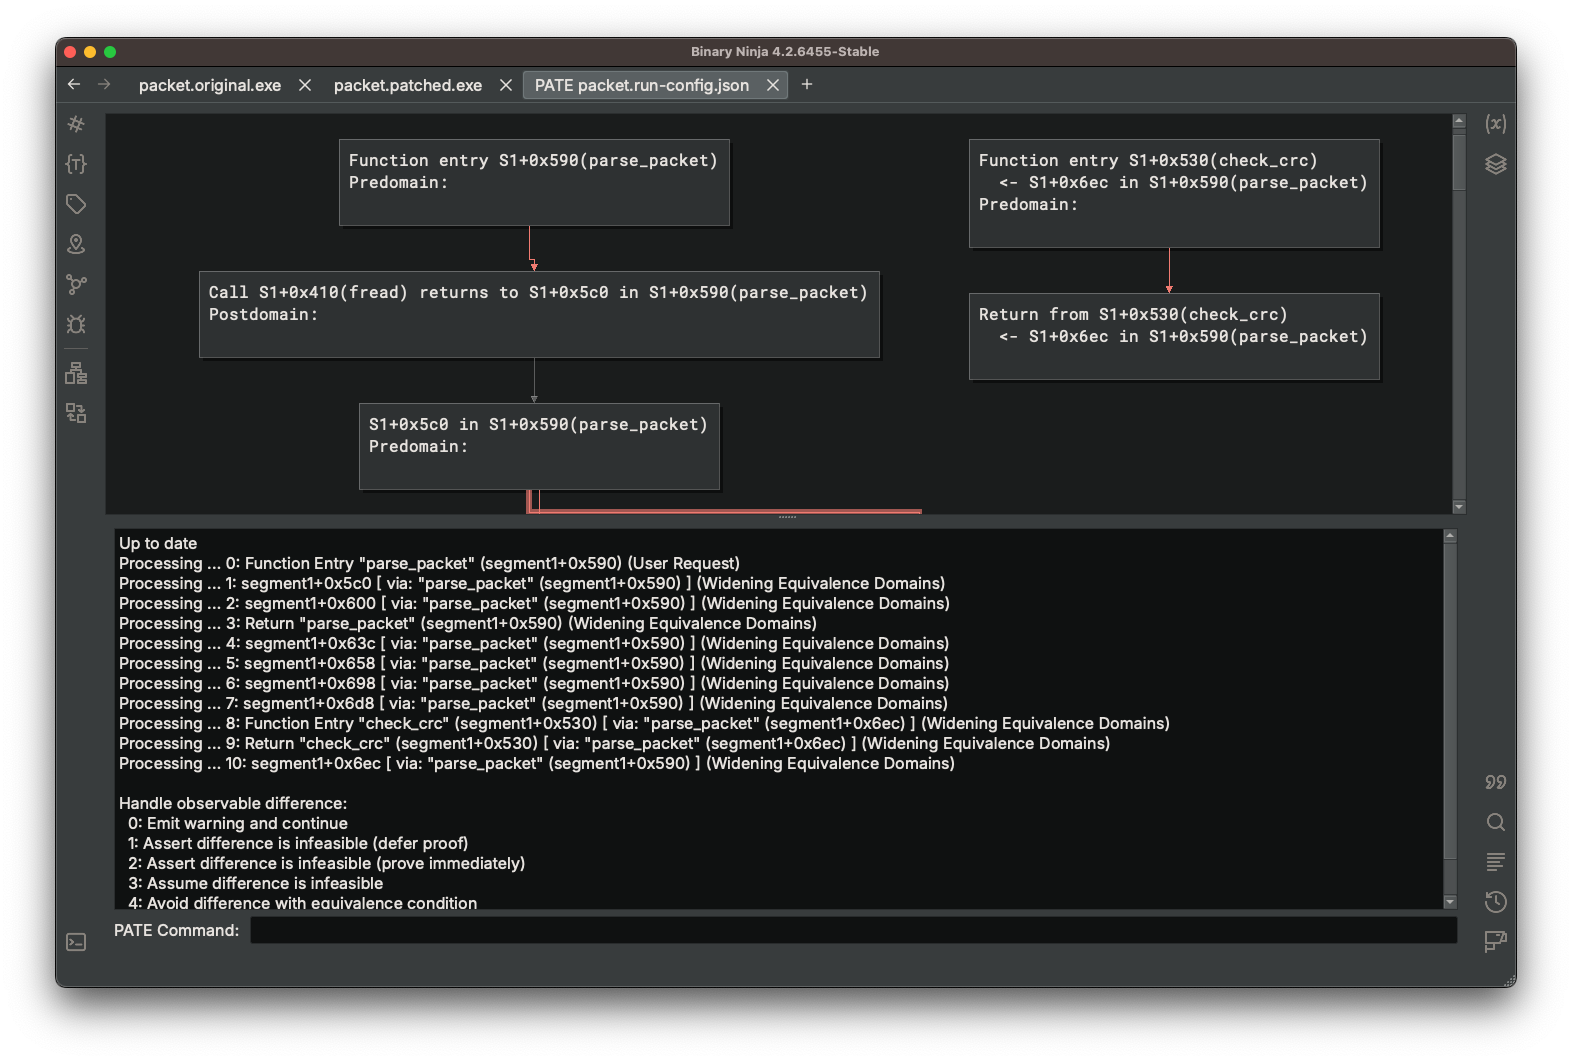
\includegraphics[width=\textwidth]{pate-binja-overview.png}
  \caption{The PATE Binary Ninja Plugin. The top region is the PATE analysis overview graph. The bottom panel is used by the operator to interact with the PATE verifier.}
  \label{fig:overview}
\end{figure}

Once installed, invoke the \pate{} plugin from the Binary Ninja ``Plugins $\rightarrow$ Pate...'' menu option.

The \pate{} plugin opens a window to select a \emph{run configuration} file in JSON format.
This file must end in the suffix \texttt{.run-config.json}.
The run configuration must contain a key-value map with the following keys:
\begin{description}
    \item[\texttt{original}] (absolute or relative) file path to the original binary
    \item[\texttt{patched}] (absolute or relative) file path to the patched binary
    \item[\texttt{args}] a list additional arguments to pass to \pate{}
\end{description}

For example, the file \texttt{tests/integration/packet/packet.run-config.json} contains:

\begin{verbatim}
  {
    "original": "exe/packet.original.exe",
    "patched": "exe/packet.patched.exe",
    "args": [
      "-s parse_packet"
    ]
  }
\end{verbatim}

After selecting the run configuration file, the \pate{} plugin will open three Binary Ninja tabs: one for each of the original and patched binaries, and a third \emph{\pate{} analysis} tab.

As shown in Figure~\ref{fig:overview}, the \pate{} analysis tab is composed of two primary regions.
The bottom portion is an interactive text view that corresponds to the terminal user interface.
The user interacts with this region through the text input field at the bottom of the window.
In the \texttt{packet.exe} example, the user enters the same commands described in Section~\ref{sec:terminal-ui} through the \texttt{Finish and view final result} step, at which point results will be rendered in the interactive Binary Ninja view.

The top portion of the \pate{} analysis tab is a graph view showing the current state of the \pate{} analysis.
When \pate{} analysis is complete (via interaction in the bottom portion), the \pate{} graph shows rectangles for each slice of the program analyzed by \pate{}.
Default-colored rectangles represent a pair of programs slices that were able to matched up between the original and patched binary.
Green rectangles represent slices present only in the original program, if any.
Blue rectangles represent slices present only in the patched program, if any.
Right-click on a rectangle for options to jump directly to the relevant program location in the appropriate tab for the corresponding binary.

A red rectangle represents the ``active'' region, where \pate{} has found an equivalence condition.
Right click and select ``Show Equivalence Condition'' to open the Equivalence Condition window.
Please see Figure~\ref{fig:equiv-cond} for an example screenshot of the equivalence condition window in the PATE Binary Ninja plugin.
An equivalence condition window includes:

\begin{itemize}
    \item the expression describing the conditions under which programs behave equivalently
    \item a generated (concretized) trace through the program(s) showing an example where the equivalence condition is met
    \item a generated (concretized) trace through the program(s) showing an example where the equivalence condition is \emph{not} met
\end{itemize}

\begin{figure}[h]
  \centering
  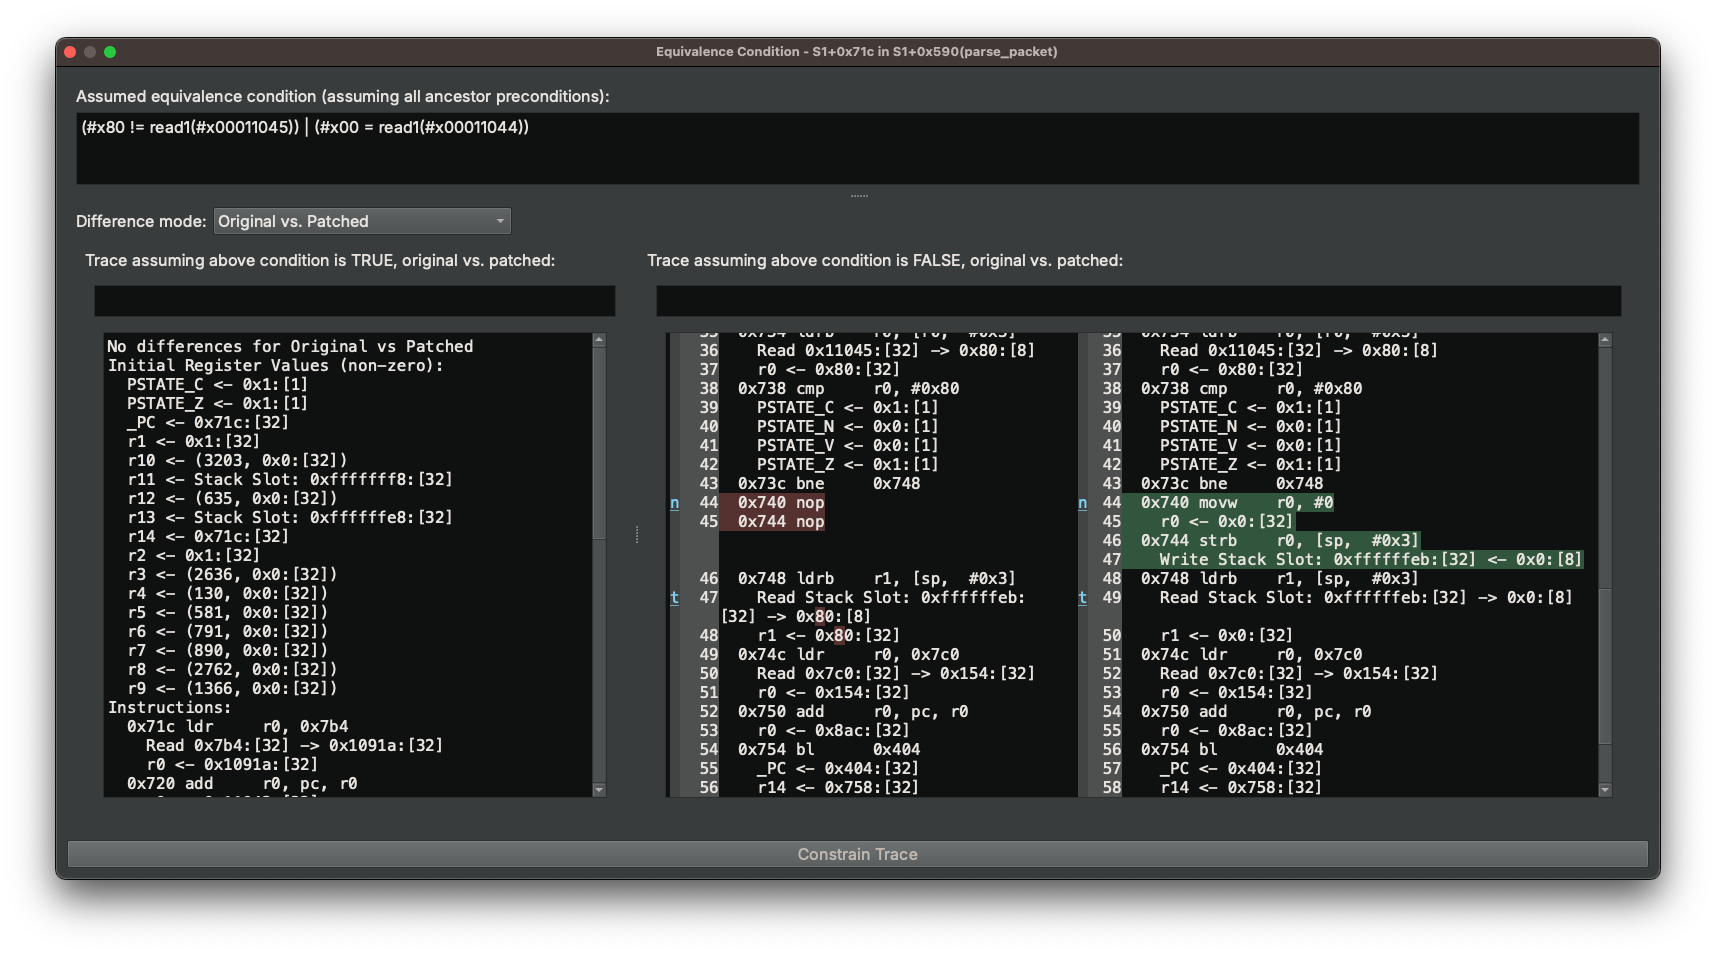
\includegraphics[width=\textwidth]{pate-binja-equiv-cond.png}
  \caption{The PATE Binary Ninja plugin equivalence condition window.}
  \label{fig:equiv-cond}
\end{figure}

Right-clicking on a rectangle in the \pate{} analysis graph and selecting ``Show Instruction Trees'' will open a new window showing basic blocks from the original program on the left and corresponding basic blocks from the patched program on the right.
At the bottom will be a linearized representation of the instruction trees in the original and patched program, with colorized diff view.
Instructions conditionally reachable through conditional control flow edges (if any) are prefixed by \texttt{+} or \texttt{-} to differentiate instructions in distinct branches.
See Figure~\ref{fig:mcad} for an example of the instruction tree view, with MCAD integration (described below).

\subsection{Trace Constraints}

The concretized traces shown in the equivalence condition window (see Figure~\ref{fig:equiv-cond}) show a pair of \emph{possible} traces
through the program slices where the equivalence condition is either met or not met. In general there may be multiple paths through
the program that may satisfy (or contradict) the equivalence condition. To observe alternative concrete traces, the final equivalence
condition may be provided \emph{trace constraints}, which restrict the values that \pate{} may choose when generating a concrete trace.
When viewing the final equivalence condition, after the verifier has finished and the user has requested the final result, the ``Constrain Trace'' 
button at the bottom becomes enabled, allowing constraints to be added to the given trace.

When ``Constrain Trace'' is clicked, the ``Trace Constraint'' window (see Figure~\ref{fig:trace-constr-empty}) appears. The
``Variable'' dropdown is populated with the memory reads from both the original and patched programs. Notably each read
is prefixed with the instruction address that the read occurred at, indicating that the constraint applies to the content
of memory at that specific program point. The user then selects a relation and enters an integer value to compare the
memory content against. Clicking ``Add'' will then add the specified constraint to the list below (see Figure~\ref{fig:trace-constr-one}).


\begin{figure}[h]
  \centering
  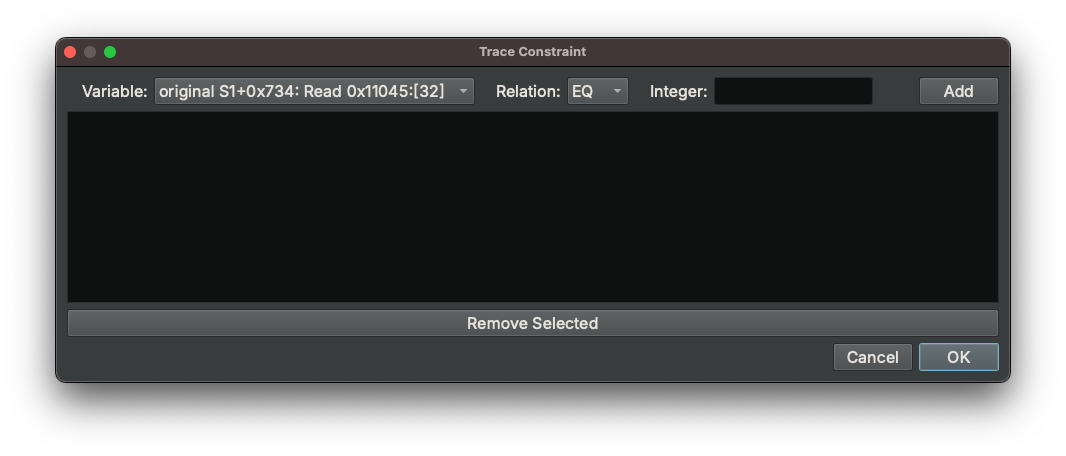
\includegraphics[width=0.8\textwidth]{pate-binja-traces2.png}
  \caption{Empty trace constraint dialogue.}
  \label{fig:trace-constr-empty}
\end{figure}

\begin{figure}[h]
  \centering
  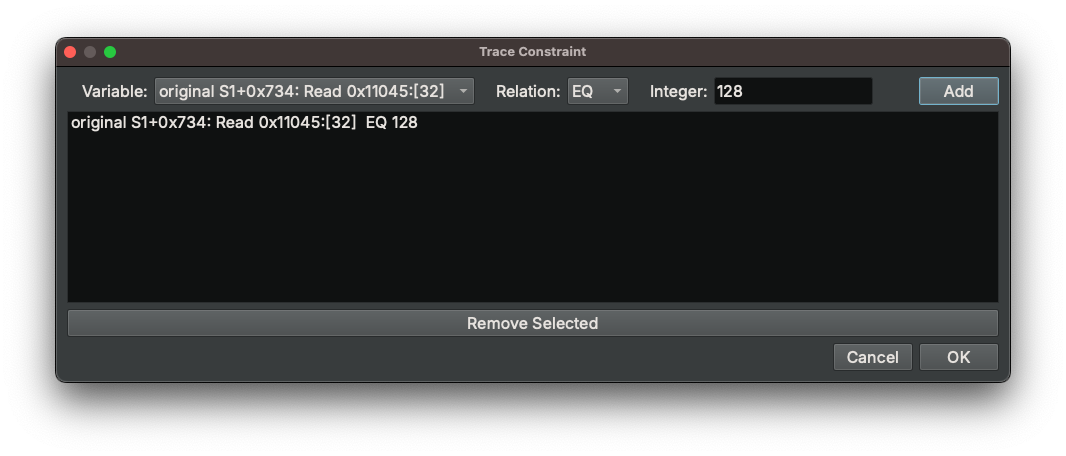
\includegraphics[width=0.8\textwidth]{pate-binja-traces3.png}
  \caption{Trace constraint dialogue with added constraint.}
  \label{fig:trace-constr-one}
\end{figure}

Multiple constraints may be added at this point, or removed via the ``Remove Constraint'' button. Once the desired set of constraints
has been provided, clicking ``OK'' will close the dialogue and present an updated equivalence condition window containing the
now-constrained traces (see Figure~\ref{fig:equiv-cond-constrained}). The equivalence condition text area lists the original equivalence condition, the user-supplied trace constraints, and the effective equivalence condition as a result of incorporating the user-provided constraints.

\begin{figure}[h]
  \centering
  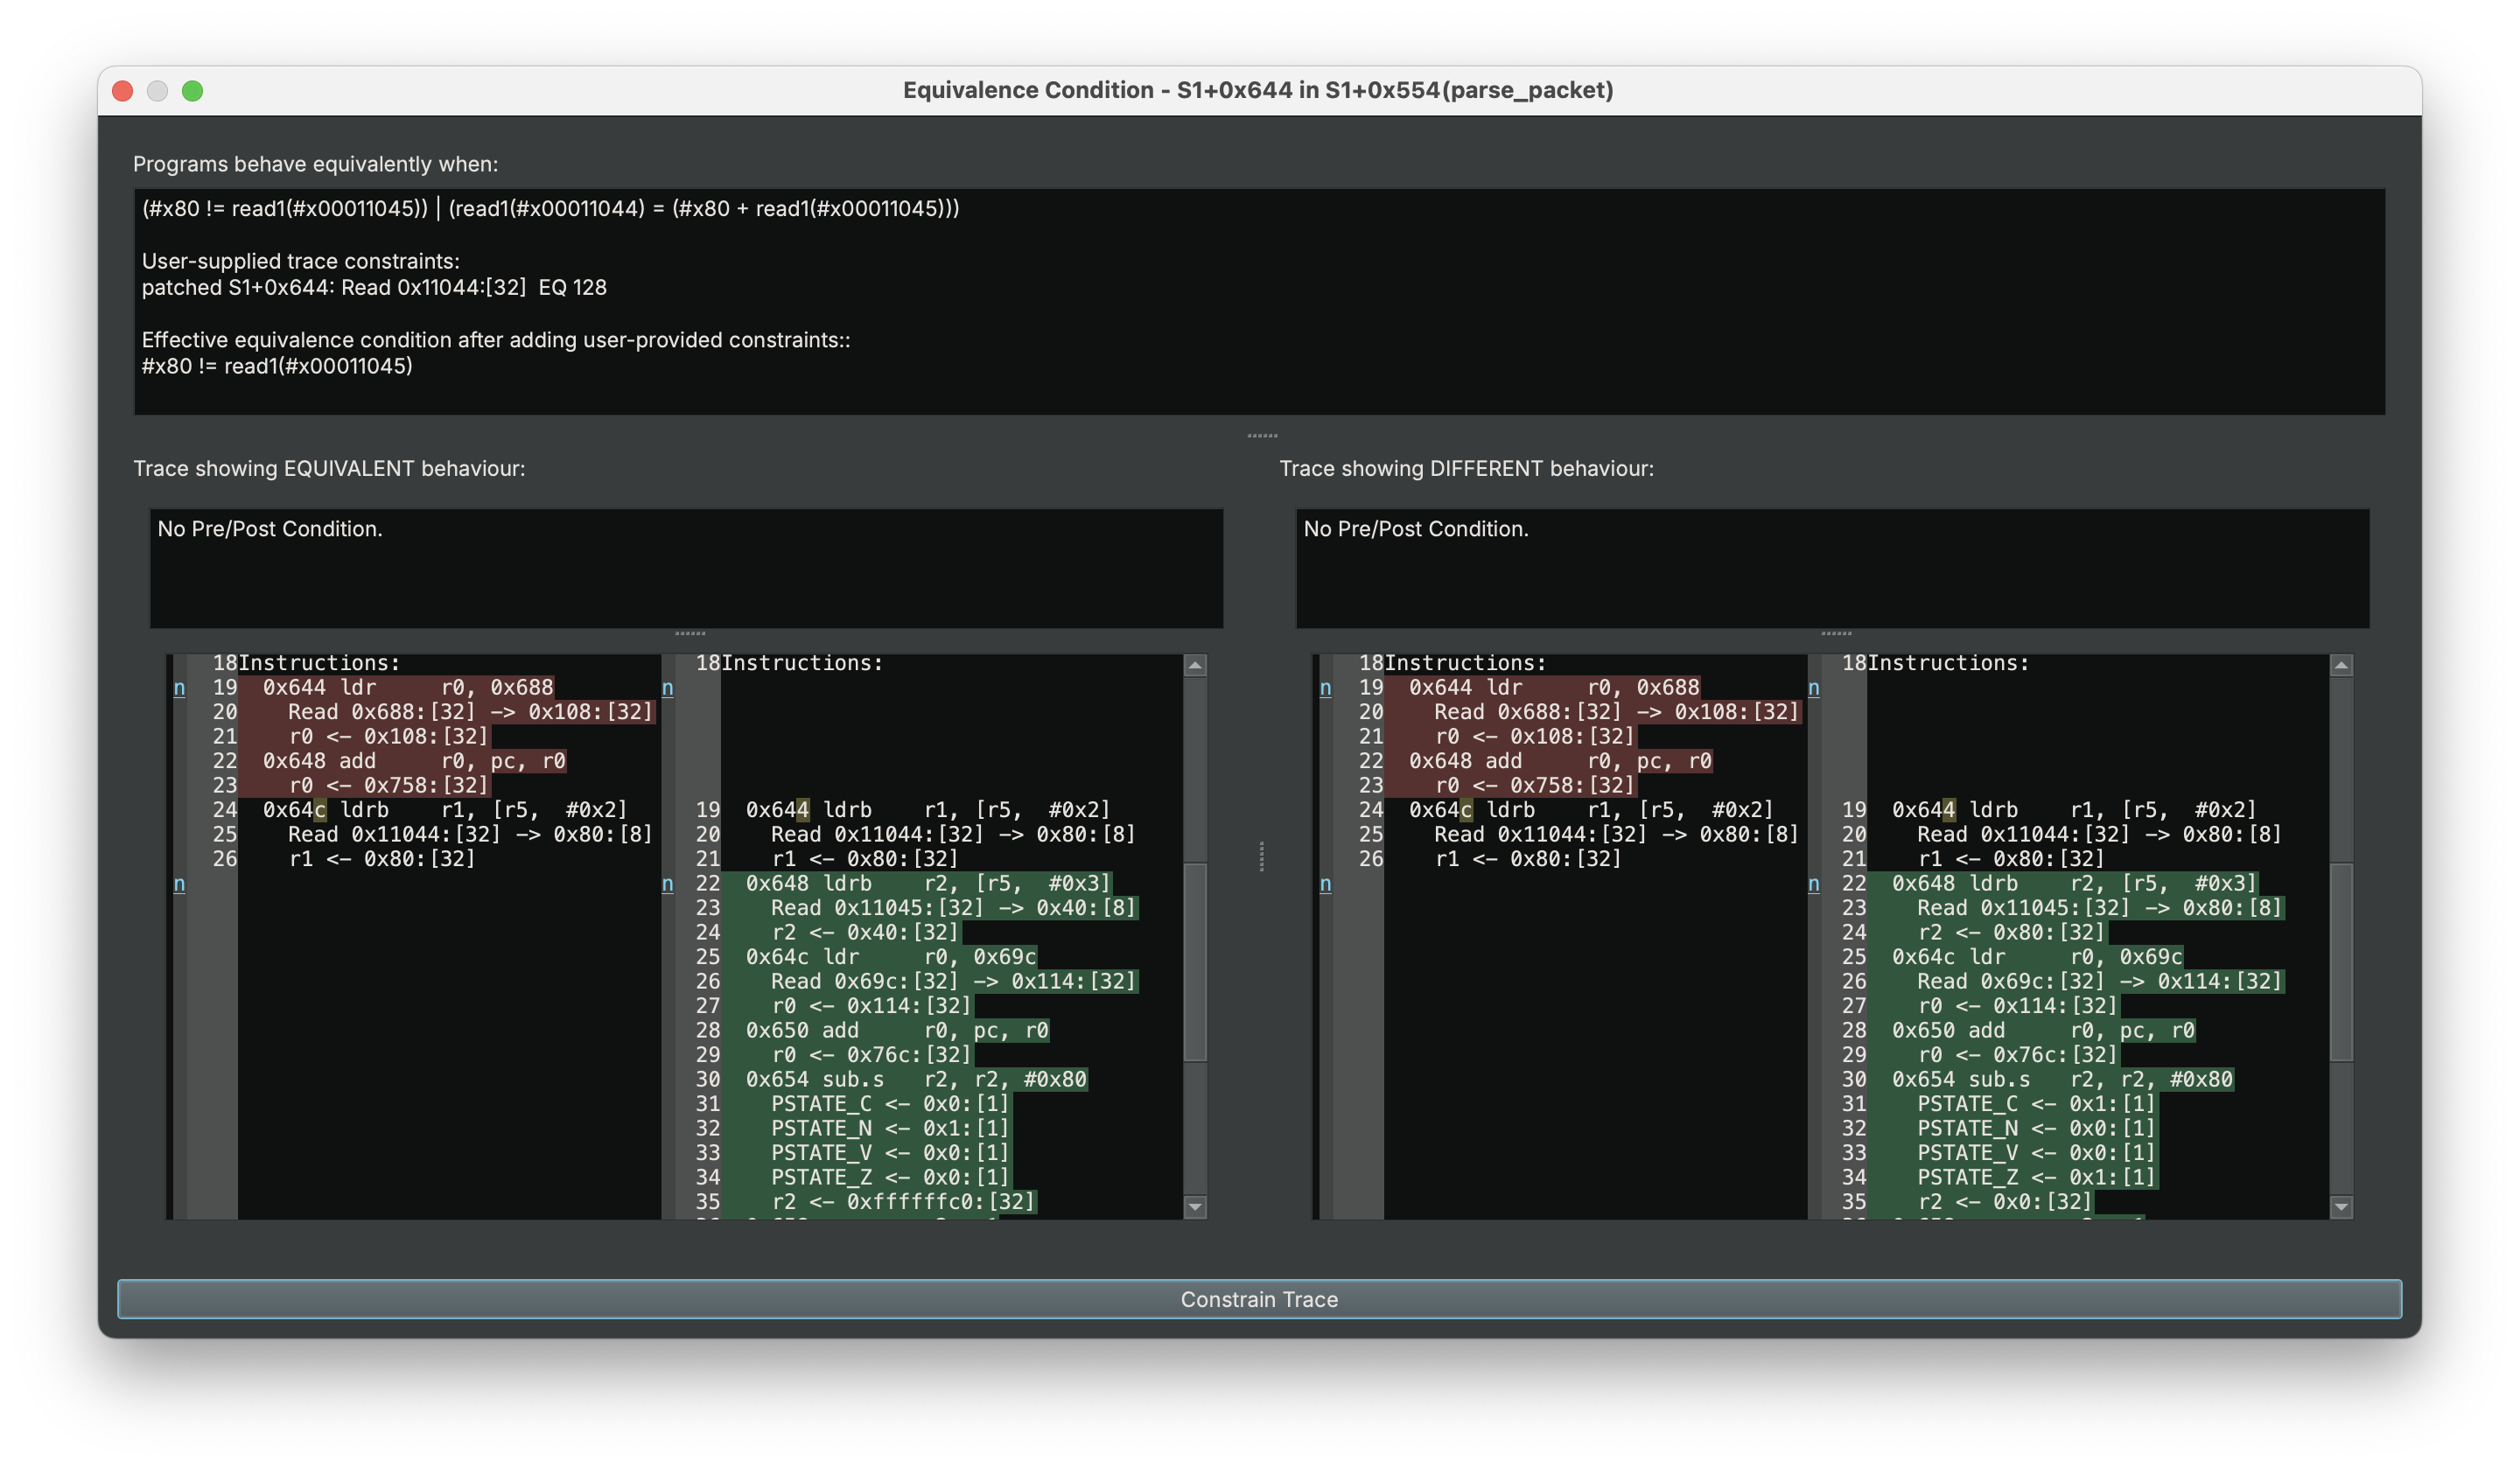
\includegraphics[width=\textwidth]{pate-binja-traces4.png}
  \caption{Expanded equivalence condition window with constrained traces.}
  \label{fig:equiv-cond-constrained}
\end{figure}

\subsection{Replays}

Executing a run configuration file with the \pate{} plugin will produce a \emph{replay} in a file named \texttt{lastrun.replay}, which can be preserved by renaming to another filename on disk.
These files cache the user input and verifier output, enabling the user to load a previous interaction with \pate{} without having to re-execute the verifier analysis.
If the user loads a replay rather than a run configuration, the process is mostly the same, except the command input field is already populated with the recorded user input, and the user just hits ``enter'' to proceed to the next step.
Editing the input commands will have no effect, as the responses are recorded in the replay file.
That is, the user cannot deviate from the pre-recorded responses from the \pate{} verifier to perform any analysis other than the one recorded.

\subsection{MCAD Integration}

MCAD\footnote{\url{https://github.com/securesystemslab/LLVM-MCA-Daemon}} is a performance analysis tool that performs static prediction of instruction timings for sequences of instructions such as those identified by \pate{}.
The details of the MCAD system is outside the scope of this user guide, but if the MCAD Docker container is available, the \pate{} Binary Ninja plugin will show MCAD-predicted cycle counts next to each instruction in the Instruction Trees view, as shown in Figure~\ref{fig:mcad}.
Use the \pate{} plugin preference option ``MCAD Docker image name'' to specify the name of the MCAD Docker container on the host in order to enable MCAD integration in the \pate{} plugin.

\begin{figure}[h]
  \centering
  \includegraphics[width=\textwidth]{pate-binja-mcad.png}
  \caption{PATE Binary Ninja MCAD integration showing predicted cycle counts (per instruction, cumulative) for instructions in original (left) and patched (right) basic blocks.}
  \label{fig:mcad}
\end{figure}